\documentclass[xcolor=table,dvipsnames,table]{beamer}
\mode<presentation>
\usetheme{boxes}
\setbeamertemplate{navigation symbols}{}
% http://www.latex-community.org/forum/viewtopic.php?f=4&t=6694
\setbeamertemplate{navigation symbols}{\raisebox{5pt}{\makebox[\paperwidth]{\hfill\makebox[10pt]{\scriptsize\insertframenumber\vspace{1ex}}}}}
%\setbeamertemplate{footline}[frame number]
\setbeamertemplate{blocks}[shadow=false]
%\setbeamercolor*{block title}{fg=structure,bg=RoyalBlue!10}
\setbeamercolor*{block title example}{fg=structure,bg=RoyalBlue!10}
%\setbeamercolor*{block title example}{fg=BrickRed,bg=Goldenrod!10}
\setbeamercolor*{block title alerted}{fg=white,bg=black}
\addtobeamertemplate{block begin}{\pgfsetfillopacity{0.8}}{\pgfsetfillopacity{1}}
%\rowcolors{0}{RoyalBlue!20}{RoyalBlue!5}
\setbeamertemplate{caption}{\raggedright\insertcaption\par}

%\DeclareGraphicsRule{*}{mps}{*}{}

\usepackage{latexsym}
\usepackage{hyperref}
\usepackage{tikz}
\usetikzlibrary{calc,shapes,arrows,shadows,shapes.callouts,shapes.arrows,chains,positioning,trees}
\usepackage{solution}
\usepackage{calc}
\usepackage{pifont}
\usepackage{algorithmic}
\usepackage{pdfcomment}
\usepackage{color}

\newcommand{\cmark}{\ding{51}}
\newcommand{\xmark}{\ding{55}}

\newcommand{\highlight}[1]{{\color{blue}{#1}}}
\newcommand{\mycite}[1]{{\color{darkgray}{\footnotesize [#1]}}}

\DeclareMathOperator*{\argmin}{arg\,min}
\DeclareMathOperator*{\argmax}{arg\,max}
\DeclareMathOperator{\sign}{sign}
\DeclareMathOperator{\cnt}{Count}

\newcounter{mycallout}

\newcommand{\callouts}[3]{%
  \stepcounter{mycallout}
  \tikz[remember picture,baseline]{\node[anchor=base,inner sep=0,outer sep=0]%
    (\themycallout) {\colorbox{#1!20}{#3}};\pause\node[overlay,rectangle callout,%
    callout relative pointer={(0cm,0.5cm)},fill=#1!20] at ($(\themycallout.south)+(-0cm,-0.7cm)$){#2};}%
    }%

\raggedright

\newcount\lecturecount
\lecturecount=0
\AtBeginLecture{%
    \advance\lecturecount by 1
    \date{}
    \begin{frame}
    \begin{center}
    \titlepage
    \ifnum\lecturecount=1
    Part \the\lecturecount: \insertlecture
    \else
    Part \the\lecturecount: \insertlecture
    \fi
    \end{center}
    \end{frame}
}

\addtobeamertemplate{block begin}{\setlength\abovedisplayskip{0pt}}

%\newcommand{\example}[1]{{\color{BrickRed!50}{#1}}}
\newcommand{\maths}[1]{{\color{RoyalBlue!50}{#1}}}
\newcommand{\reference}[1]{{\color{RoyalBlue!30}\tiny [from #1]}}
\newcommand{\koehnref}{\reference{\href{http://www.statmt.org/book}{P.Koehn SMT book slides}}}


\begin{document}

\title{\color{MidnightBlue}Natural Language Processing}

\author{Anoop Sarkar \\ {\color{RoyalBlue!70}{\href{http://anoopsarkar.github.io/nlp-class}{anoopsarkar.github.io/nlp-class}}}}
\institute{\color{BrickRed}Simon Fraser University}
%\date{}
     
{
\addtocounter{framenumber}{-1}
\begin{frame}
\begin{center}
\vspace{8mm}

\includegraphics[scale=0.35]{figures/natlang-cky-logo}
\end{center}
\titlepage
\end{frame}
}



\lecture{Neural Language Models}{}
\section{Long distance dependencies}

\begin{frame}
\frametitle{Long distance dependencies}
\begin{block}{Example}
\begin{itemize}[<+->]
\item {\color{blue} He} doesn't have very much confidence in {\color{blue} himself}
\item {\color{blue} She} doesn't have very much confidence in {\color{blue} herself}
\end{itemize}

\pause
\end{block}
\begin{block}{n-gram Language Models: $P(w_i \mid w_{i-n+1}^{i-1})$}
\begin{eqnarray*}
P(\text{himself} &\mid& \text{confidence}, \text{in} ) \\
P(\text{herself} &\mid& \text{confidence}, \text{in} ) 
\end{eqnarray*}
\end{block}

\pause
\begin{block}{What we want: $P(w_i \mid w_{<i})$}
\begin{eqnarray*}
P(\text{himself} &\mid& \text{confidence}, \ldots, \text{him} ) \\
P(\text{herself} &\mid& \text{confidence}, \ldots, \text{her} ) 
\end{eqnarray*}
\end{block}
\end{frame}

\begin{frame}{Long distance dependencies}
\framesubtitle{Other examples}	
\begin{itemize}[<+->]
	\item \textbf{Selectional preferences}: \textit{I ate lunch with a {\color{blue} fork}} vs.\ \textit{I ate lunch with a {\color{blue} backpack}}
	\item \textbf{Topic}: \textit{Babe Ruth was able to touch the home {\color{blue} plate} yet again} vs.\ \textit{Lucy was able to touch the home {\color{blue} audiences} with her humour}
	\item \textbf{Register}: Consistency of register in the entire sentence, e.g.\ informal (Twitter) vs.\ formal (scientific articles)
\end{itemize}
\end{frame}

\begin{frame}
\frametitle{Language Models}
\begin{block}{Chain Rule and ignore some history: the trigram model}
\begin{eqnarray*}
\lefteqn{p(w_1, \ldots, w_n) } \\
&\approx& p(w_1) p(w_2 \mid w_1) p(w_3 \mid w_1, w_2) \ldots p(w_n \mid w_{n-2}, w_{n-1}) \\
&\approx& \prod_{t} p(w_{t+1} \mid w_{t-1}, w_t)
\end{eqnarray*}
\end{block}
\pause
\begin{block}{How can we address the long-distance issues?}
\begin{itemize}
\item Skip $n$-gram models. Skip an arbitrary distance for $n$-gram context.
\item Variable $n$ in $n$-gram models that is adaptive
\item {\bf Problems}: Still "all or nothing". Categorical rather than soft.
\end{itemize}
\end{block}
\end{frame}

\begin{frame}
\frametitle{Neural Language Models}
\begin{block}{Use Chain rule and approximate using a neural network}
\[ p(w_1, \ldots, w_n) \approx \prod_{t} p(w_{t+1} \mid \underbrace{\phi(w_1, \ldots, w_t)}_{\text{capture history with vector $s(t)$}}) \]
\end{block}
\pause
\begin{block}{Recurrent Neural Network}
\begin{itemize}[<+->]
	\item Let $y$ be the output $w_{t+1}$ for current word $w_t$ and history $w_1, \ldots, w_t$
	\item $s(t) = f(U_{xh} \cdot w(t) + W_{hh} \cdot s(t-1))$ where $f$ is sigmoid
	\item $s(t)$ encapsulates history using single vector of size $h$
	\item Output word at time step $w_{t+1}$ is provided by $y(t)$
	\item $y(t) = g(V_{hs} s(t))$ where $g$ is softmax
\end{itemize}
\end{block}
\end{frame}

\begin{frame}{Neural Language Models}
\framesubtitle{Recurrent Neural Network}
\begin{block}{Computational Graph for an RNN Language Model}
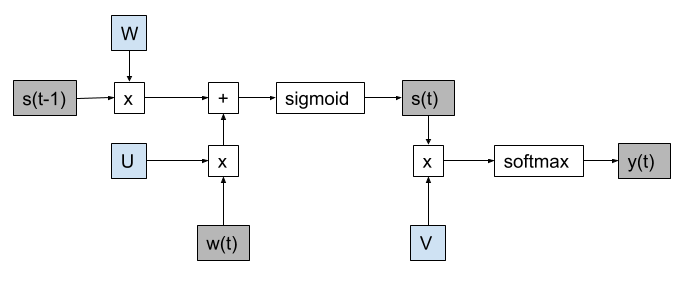
\includegraphics[scale=0.45]{figures/mikolovrnn-graph.png}
\end{block}
\end{frame}


\section*{Acknowledgements}

\begin{frame}
\centering
\begin{alertblock}{Acknowledgements}
Many slides borrowed or inspired from lecture notes by Michael Collins, Chris Dyer, Kevin Knight, Philipp Koehn, Adam Lopez, Graham Neubig and Luke Zettlemoyer from their NLP course materials. 

\bigskip

All mistakes are my own.

\bigskip

A big thank you to all the students who read through these notes and helped me improve them.

\end{alertblock}
\end{frame}



\end{document}
